\subsection{Game Engine Modul Test}

Nedestående præsenteres en delvis tabel for alle klasser testet som led i Game Engine. De vigtigste er GameController, CombatController og DiceRoller. Dice danner ``Core Mechanics'' for spillet.

Interessant nok ses her at GameController fejler sine test grundet at der ikke er skrevet test til mange af GameControllerens ansvars punkter.

\begin{center}
  \captionof{table}{Her Ses en komplet liste over alle test foretages på
                  Game Engine komponenter, med kommentar til deres resultater
                  og en endelig vurdering af test resultaterne.}
  \vspace{-1em}
  \label{tab:testEngine}
  \begin{longtable}{|l|p{0.25\linewidth}|p{0.25\linewidth}|l|}
  \hline
  \multicolumn{4}{|c|}{\textbf{Game Engine GodkendelsesTabel}} \\ \hline
  \textbf{Komponent under test} & \textbf{Forventet Adfærd} & \textbf{Kommentar} & \textbf{Test Resultat} \\ \hline
  Game Controller
  &
    \begin{enumerate}
      \item \begin{flushleft} Kan skifte Player til Nyt Room \end{flushleft}
      \item \begin{flushleft} Kan samle Item op fra Room  \end{flushleft}
      \item \begin{flushleft} Kan save Game \end{flushleft}
      \item \begin{flushleft} Kan loaded Games \end{flushleft}
      \item \begin{flushleft} Kan eliminere Enemy fra Game \end{flushleft}
      \item \begin{flushleft} Kan reset Game \end{flushleft}
      \item \begin{flushleft} Kan anskaffe Room description \end{flushleft}
    \end{enumerate}
  &
  \flushleft 
  Game Controller er kun test for at skifte til nyt Room, dette betyder at der 
  ikke kan stilles garanti for at resterende implementeringer af load- og save game
  osv. fungere som ønsket. Disse ting er svagt testet gennem visuelt trial and error
  test, men da der ikke er skrevet nogen specifikke test til dem Fejler 
  GameControlleren sin komponent test.
  &
  FAIL
  \\ \hline
  Combat Controller
  &
  \begin{enumerate}
    \item \begin{flushleft} Kan Håndtere Combat Rounds \end{flushleft}
    \item \begin{flushleft} Kan håndtere at Player løber væk fra Combat \end{flushleft}
  \end{enumerate}
  &
  \flushleft
  Combat controller kan håndtere at spilleren løber fra combat og at Player indgår i combat.
  CombatController kan stille garanti for at combat sker i den rigtige orden og at hverken
  spiller eller enemy kan angribe hvis denne er død.
  Ydmere stiller den garanti for at både enemy og spiller kan lave ``critial hits'' hvis dice
  rolleren slår 20.
  &
  OK
  \\ \hline
  DiceRoller
  &
  \begin{enumerate}
    \item \begin{flushleft} Kan emulerer et kast med en N siddet terning \end{flushleft}
    \item \begin{flushleft} Kan emulerer N kast med en M siddet terning \end{flushleft}
  \end{enumerate}
  &
  \flushleft
  DiceRoller Kan emulere et eller flere terninge kast med samme antal sidder. Denne kan
  ydmere stille krav for at fordellingen af disse terningekast har en normal distribution 
  og dermed er alle udfald lige sandsynlige.
  &
  OK
  \\ \hline
  \end{longtable}
  \addtocounter{table}{-1}
\end{center}

\subsubsection{Test Resultater for Game Engine}
Nedestående vises kort resultatet for Game Engine test \parencite[Section 12.2.1][]{TekniskBilag}, når de alle køres via visual
studio. Som det kan ses så er alle testene succesfulde, hvilket giver hvis garanti for at
game engine opfører sig som specificeret i kravspecifikationerne og i de implementerede interfaces.

\begin{figure}[H]
  \centering
  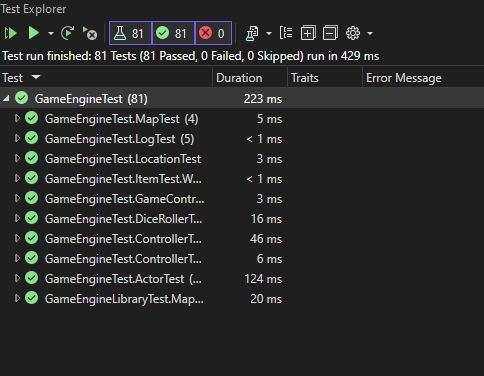
\includegraphics[scale=0.4]{02-body/Images/Test Results.png}
    \caption{Alle skrevene test til Game Engine passer, hvilket hjælper med at give vished
          om at Game Engine udfører dens funktionalitet, som det er beskrevet i kravene.
          Dette siges da alle testene er skrevet på baggrund af kravene som black-box tests
          og ikke som white-box test efter implementeringen.}
  \label{fig:TestResultsGameEngine}
\end{figure}

\noindent Disse resultater giver en god sikkerhed for at game controlleren fungere som den skal. Desværre er 
mængden af test mangelfuld og derfor kan der ikke stille nogen garanti for at game engine fungere
som forventet.

\newpage
